\documentclass{article}

% Language setting
% Replace `english' with e.g. `spanish' to change the document language
\usepackage[french]{babel}
\usepackage[fleqn]{amsmath} % Aligner les équations à gauche


% Set page size and margins
% Replace `letterpaper' with`a4paper' for UK/EU standard size
\usepackage[letterpaper,top=2cm,bottom=2cm,left=3cm,right=3cm,marginparwidth=1.75cm]{geometry}

% Useful packages
\usepackage{amsmath}
\usepackage{graphicx}
\usepackage[colorlinks=true, allcolors=blue]{hyperref}

\title{TD1}
\author{IPESUP - PC }
\date{8 Novembre 2023}

\begin{document}
\maketitle


\section{Rappels de cours}
Les équations de Maxwell locales :\\
\\
\par \(div(\vec{E})=\frac{\rho}{\epsilon_0}\) \\
\par \(\vec{rot}(\vec{E}) = -\frac{\partial\vec{B}}{\partial t}\)\\
\par \(div(\vec{B})=0\) \\
\par \(\vec{rot}(\vec{B}) = \mu_0 \vec{j} + \frac{1}{c^2}\frac{\partial\vec{E}}{\partial t}\)\\

Les équations de Maxwell sous forme intégrale :\\


$\oint_S \vec{E} \cdot d\vec{A} = \frac{1}{\varepsilon_0} \int_V \rho \, dV$\\

$\oint_C \vec{B} \cdot d\vec{l} = \mu_0 \int_S \vec{j} \cdot d\vec{A} + \mu_0\varepsilon_0 \frac{d}{dt}\int_S \vec{E} \cdot d\vec{A}$
\\[0.2cm]

 La vitesse de phase vaut $v_\phi = \frac{\omega}{\lVert\vec{k}\rVert}$. Si elle dépend de $\omega$, alors on dit qu'il y a dispersion. 
 \\[0.2cm]
   \par La vitesse de groupe vaut $v_g=\frac{d\omega}{dk}$\\[0.2cm]
 \par Le vecteur de Poynting vaut $\vec{\Pi} = \vec{E}\wedge \frac{\vec{B}}{\mu_0}$
\section{Calcul de champ}
On considère un fil conducteur parcouru par un courant I pénétrant dans un conducteur isotrope occupant tout l'espace des $z>0$. Déterminer le champ magnétique dans le concucteur illimité $z>0$. 
\begin{figure}[h]
  \centering
  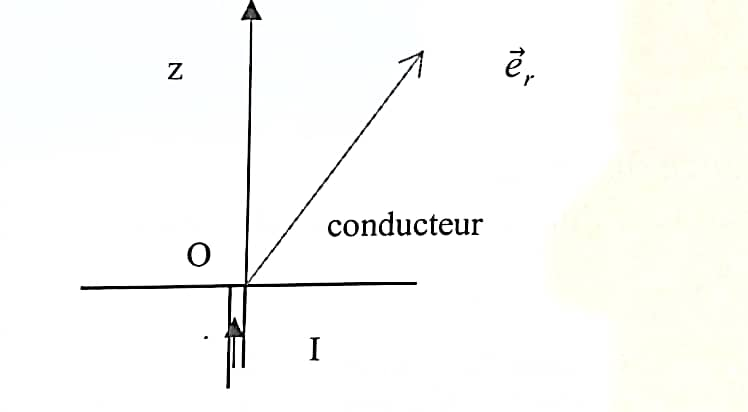
\includegraphics[width=0.4\textwidth]{schéma_conducteur_isotrope.jpg}
  \label{fig:image1}
\end{figure}
\\[1cm]
\section{OPPH de direction quelconque}
On considère une onde électromagnétique se propageant dans le vide dont le champ électrique vaut:\\[0.2cm]
$\vec{E}=E_x\vec{u_x}+E_y\vec{u_y}$ avec $E_x=exp[i(\frac{k}{3}(2x+2y+z)-\omega t)]$\\[0.2cm]
On note $\lambda=6.10^{-7}m $ la longueur d'onde
\begin {enumerate}
\item Calculer la fréquence de l'onde. A quel domaine du spectre électromagnétique l'onde appartient-elle ? 
\item Calculer la valeur numérique de k.
\item Déterminer l'équation cartésienne d'un plan d'onde. 
\item Déterminer la valeur de $E_y$ en fonction de $E_x$
\item Calculer le champ $\vec{B}$ associé. 
\item Calculer la densité moyenne d'énergie électromagnétique de l'onde. 
\item Calculer le vecteur de Poynting et sa moyenne temporelle.
\end{enumerate}

\section{Puissance rayonnée par une onde sphérique}
On se place en coordonnées sphériques. 
On considère une onde sphérique de la forme $\vec{E}(M,t)=\frac{A}{r} cos(\omega t - k r ) \vec{e_\theta})$

\begin{enumerate}
    \item Montrer que cette onde est solution de l'équation d'Alembert.
    \item Déterminer le champ$ \vec{B}$ dans tout l'espace.
    \item Calculer le vecteur de Poynting associé à cette onde puis en déduire la puissance rayonnée à travers une sphère centrée en O et de rayon $R$. 
    \item Justifier la dépendance en $\frac{1}{r}$ de l'amplitude de $\vec{E}$
    
\end{enumerate}

En coordonnées sphériques, le laplacien d'un champ scalaire $f$ vaut: \\[0.1cm]
\par $\Delta f = \frac{1}{r^2} \frac{\partial}{\partial r} \left(r^2 \frac{\partial f}{\partial r}\right) + \frac{1}{r^2 \sin \theta} \frac{\partial}{\partial \theta} \left(\sin \theta \frac{\partial f}{\partial \theta}\right) + \frac{1}{r^2 \sin^2 \theta} \frac{\partial^2 f}{\partial \phi^2}
$
\\[0.1cm]

Le rotationnel en coordonnées sphériques vaut:\\


$\vec{rot}(\vec{F}(r, \theta, \phi)) = \frac{1}{r \sin \theta} \left(\frac{\partial(\sin \theta F_\phi)}{\partial \theta} - \frac{\partial F_\theta}{\partial \phi}\right) \vec{e}_r + \frac{1}{r} \left(\frac{1}{\sin \theta} \frac{\partial F_r}{\partial \phi} - \frac{\partial(r F_{\phi})}{\partial r}\right) \vec{e}_\theta + \frac{1}{r} \left(\frac{\partial(rF_\theta)}{\partial r} - \frac{\partial F_r}{\partial \theta}\right) \vec{e}_\phi
$
\end{document}



\section{Exercice 1}

\section{Exercice 2}

\section{Exercice 3}

\section{ Formulaire }

\end{document}